%  !TeX  root  =  user_guide.tex

\section{Plugin OpenStreetMap}\label{plugins_osm}

% when the revision of a section has been finalized,
% comment out the following line:
% \updatedisclaimer

Il progetto OpenStreetMap (OSM) si sta ampiamente diffondendo, sopratutto in quei paesi dove 
non si hanno a disposizione dati geografici liberi.
L'obiettivo di OSM è la creazione di una mappa aggiornabile e libera del mondo a partire da
dati GPS, foto aeree e conoscenza locale.
Per supportare tale obiettivo, QGIS mette a disposizione un plugin che permette di lavorare 
con i dati OSM.

Il plugin offre le principali funzionalità per la manipolazione dei dati OSM; download/upload dei dati,
salvataggio, modifica. 
Nell'implementare il plugin, il team di sviluppo ha preso ispirazione dagli editor di 
dati OSM esistenti, nell'obiettivo di combinare le loro funzionalità in un unico prodotto.

La sezione seguente, fornisce una breve introduzione ai principi del progetto OSM.
Parti del paragrafo che segue sono riprese dal sito web di OpenStreetMap: \url{http://www.openstreetmap.org}.

\minisec{Il progetto OpenStreetMap}

L'obiettivo di OSM è la creazione di una mappa aggiornabile e libera del mondo a partire da
dati GPS, foto aeree e conoscenza locale.
Il progetto è stato iniziato perché molti dati geografici hanno restrizioni legali e tecniche,
che impediscono il loro utilizzo in maniera creativa e produttiva. 
I dati di OSM e le immagini da essi derivate sono, invece, disponibili sotto la licenza 
Creative Commons Attribution ShareAlike 2.0.

\begin{figure}[ht]
   \centering
   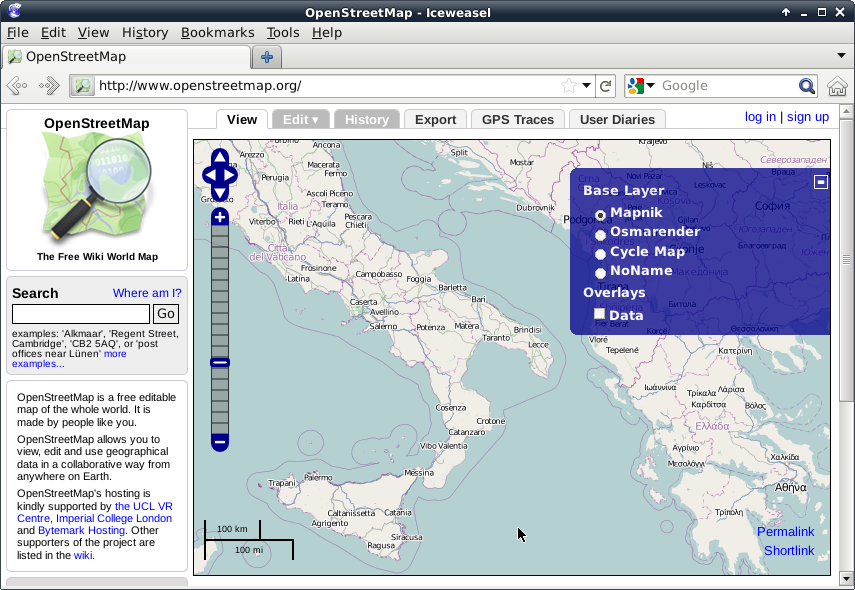
\includegraphics[clip=true, width=13cm]{osmweb}
   \caption{Dati OpenStreetMap nel web \nixcaption}\label{fig:osmweb}
\end{figure}

OpenStreetMap si è ispirato a progetti tipo Wikipedia: la mappa di OSM (Figura \ref{fig:osmweb}) 
mostra una ben visibile scheda \tab{Edit} e viene mantenuto lo storico di tutte 
le modifiche effettuate. Gli utenti registrati possono caricare track GPS ed editare dati 
vettoriali utilizzando gli editor disponibili.

La 'primitiva dati' di OSM è una classe oggetto che può essere memorizzata via API nel server.
I tre tipi di dati supportati sono: \textbf{Node} (nodo), \textbf{Way} (via)
e \textbf{Relation} (relazione). Non esiste una primitiva dati di tipo area: 'way' chiuse ed 
opportunamente etichettate vengono gestite come aree.

\begin{itemize}[label=--]
\item Un \textbf{nodo} è una coppia latitudine/longitudine di coordinate: è il punto di partenza 
per la costruzione di tutti gli altri elementi ed è un elemento esso stesso 
(POI - Point of Interest).
\item Una \textbf{via} è un elenco di almeno due nodi che descrivono un elemento 
lineare, es. una strada. I nodi possono essere parte di più 'vie'.
\item Una \textbf{relazione} è un gruppo di zero o più primitive 
con ruoli associati. È usata per specificare il rapporto tra oggetti e per modellare un 
oggetto astratto.
\end{itemize}

Queste primitive sono usate per definire diversi elementi logici di una mappa 
('Point Of Interest', 'Street', 'Tram Line', 'Bus Stop' etc.).
Gli elementi di mappa sono ben noti nella comunità OSM e sono memorizzati 
tramite etichette basate su una chiave ed un valore. 
I dati OSM sono solitamente distribuiti in formato XML, che è usato anche per 
la comunizazione con i server OSM.

\minisec{QGIS - Connessione a OSM}\label{qgis-osm-connection}

La prima parte di questa sezione descrive come le primitive OSM sono visualizzate QGIS.
Come precedentemente descritto, i dati OSM consistono di 'node', 'way' e 'relation'. In 
QGIS le tre primitive vengono visualizzate con differenti tipi di layer: punti, linee, 
poligoni. Non è possibile rimuovere uno di questi layer e lavorare con i rimanenti.

\begin{itemize}[label=--]
\item Un \textbf{layer di punti} visualizza i soli elementi di tipo 'node' che non sono 
parte di 'way'. 
\item Un \textbf{layer di linee} visualizza gli elementi di tipo 'way' non chiusi (a formare 
poligoni): nessuna delle 'way' inizia e finisce nello stesso 'node'.
\item Un \textbf{layer di poligoni} visualizza tutte le 'way' non incluse nel layer di linee, 
cioè le linee chiuse.
\end{itemize}

Le \textbf{Relation} non sono visualizzate come layer vettoriale in quanto servono a definire 
le connessioni tra le altre primitive dati: dopo che un punto/linea/poligono è individuato 
sulla mappa, il plugin mostra un elenco delle relazioni di cui l'elemento è parte.

Ha richiesto un notevole impegno tentare di collegare i dati OSM con gli strumenti di modifica standard 
di QGIS. Tali strumenti sono fatti per modificare un singolo layer alla volta, a prescindere 
dal tipo di elemento: ciò significa che se i dati OSM venissero caricati in QGIS tramite il plugin, 
sarebbe teoricamente possibile modificare i layer di punti, di linee, di poligoni separatamente con 
gli strumenti standard.  

Un layer di linee consiste di due diversi tipi di elementi OSM, 'node' e 'way'. Nel formato OSM, 
una 'way' è composta di 'node'; se si modifica un layer di linee, ad esempio cambiando la 
forma di qualche elemento, tale azione influenza anche i 'node' che sono parte dello stesso.

Gli strumenti di modifica standard di QGIS non sono in grado di gestire tale tipo di relazioni 
e inviare correttamente le modifiche alla banca dati OSM. Il layer di linee non tiene traccia 
di quali 'node' sono parte di quale 'way': lo stesso problema si ha con i layer di poligoni.

Per tale ragione, il plugin OSM necessita dei propri strumenti di modifica, tramite i quali le modifiche 
ai layer OSM vengono gestiti correttamente. 
Gli strumenti di modifica del plugin permettono di creare/muovere/eliminare punti, linee, poligoni, 
relazioni.

\textbf{Nota:} Per creare una connessione tra il plugin OSM e gli strumenti di modifica standard 
di QGIS, sarebbero necessarie modifiche a livello di codice.

\subsection{Installazione}

Il plugin OpenStreetMap è un plugin core di QGIS. Se il supporto a python è abilitato, 
il plugin può essere attivato nel gestore di plugin, come descritto nella Sezione \ref{sec:load_core_plugin}.

\subsection{Interfaccia utente di base}

In seguito all'attivazione del plugin ed al caricamento di alcuni dati, nel menu delle barra degli strumenti 
di QGIS appaiono diverse icone OSM, insieme alla nuova componente grafica mostrata in Figura \ref{fig:osmwidget}:

\begin{figure}[ht]
   \centering
   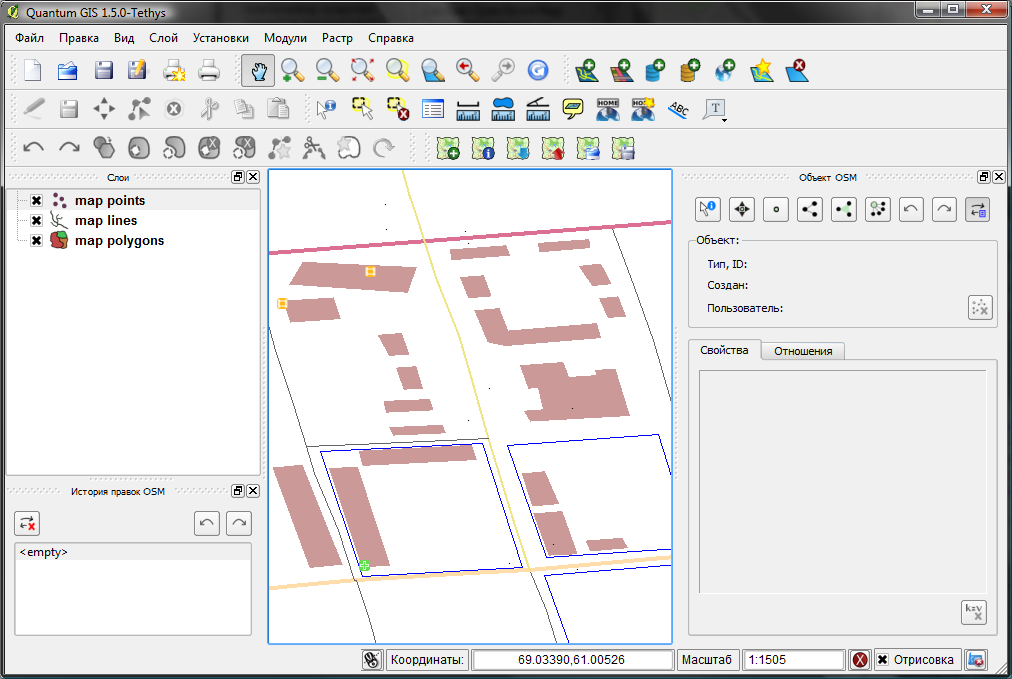
\includegraphics[clip=true, width=10cm]{osm_widgets}
   \caption{Interfaccia del plugin OSM \wincaption}\label{fig:osmwidget}
\end{figure}

\minisec{Pannello Elemento OSM}

Il pannello Elemento OSM consente di identificare gli elementi OSM, fornendo informazioni sul tipo di 
elemento, sul suo identificatore, su chi l'ha modificato e quando: in esso sono, inoltre, presenti 
tutti gli strumenti di modifica, di seguito descritti. 
Il pannello è inizialmente disabilitato: viene abilitato al caricamento di dati OSM. 

\minisec{Pannello Storico modifiche OSM}

Il pannello 'Storico modifiche OSM' permette di annullare/ripristinare le modifiche più recenti. Oltre ai pulsanti classici 
di annulla/ripristina, mostra una lista con una breve descrizione delle operazioni di modifica più recenti.
Il pannello può essere attivato con l'apposito pulsante del pannello Elemento OSM.

\minisec{Icone nel menu della barra degli strumenti}

\begin{description}
\item \toolbtntwo{osm_load}{Load OSM from file}: permette di caricare dati da file OSM in XML.
\item \toolbtntwo{osm_featureManager}{Show/Hide OSM Feature Manager}: permette di visualizzare/nascondere 
l'Elemento OSM 
\item \toolbtntwo{osm_download}{Download OSM data}: per scaricare dati dai server di OpenStreetMap.
\item \toolbtntwo{osm_upload}{Upload OSM data}: permette di salvare le modifiche ai dati correnti.
\item \toolbtntwo{osm_import}{Import data from a layer}: permette di importare dati da layer vettoriali: è necessario 
caricare almeno un layer vettoriale e selezionati alcuni dati OSM.
\item \toolbtntwo{osm_save}{Save OSM to file}: permette di salvare dati OSM in un file XML.
\end{description}

\subsection{Caricare dati OSM}

La prima azione dopo aver lanciato il plugin consiste nell'aprire alcuni dati da un file OSM: i dati OSM possono 
essere importati come shapefile o scaricati dai server di OSM.
Qui di seguito ci si riferisce alla prima modalità

Per caricare dati da un file utilizzare l'icona \toolbtntwo{osm_load}{Load OSM from file}: se l'icona non 
è visualizzata, il plugin potrebbe essere disabilitato. Abilitarlo da 
\mainmenuopt{Visualizza} \arrow \mainmenuopt{Barre degli strumenti} \arrow \dropmenuopt{OpenStreetMap}.

\begin{figure}[ht]
   \centering
   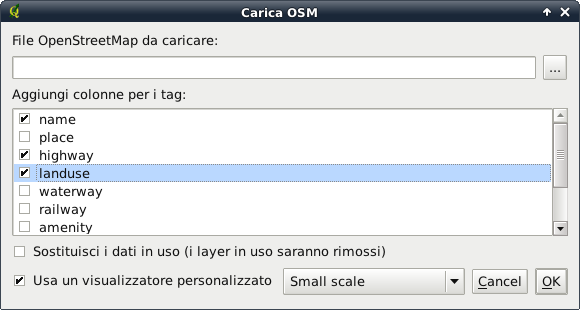
\includegraphics[clip=true, width=10cm]{osmloaddialog}
   \caption{Finestra di dialogo per caricare dati OSM \nixcaption}\label{fig:osmload}
\end{figure}

\begin{description}
\item \textbf{File OpenStreetMap da caricare}: selezionare il file .osm da cui si vogliono caricare i dati.
\item \textbf{Aggiungi colonne per i tag}: permette di creare una connessione tra OSM e QGIS. Ogni elemento
OSM ha alcune etichette (coppia chiave-valore) che ne definiscono le proprietà: anche ogni elemento di un layer 
vettoriale di QGIS ha i propri attributi (chiave-valore). 
Con questa opzione è possibile definire quali proprietà degli oggetti OSM devono essere visibili quando si visualizzano 
le informazioni dell'elemento QGIS.
\item \textbf{Sostituisci i dati in uso}: attivando l'opzione, i nuovi dati sostituiscono quelli su cui l'utente 
stava precedentemente lavorando. Se si sta caricando dati OSM per la prima volta, l'opzione non è attiva.
\item \textbf{Usa un visualizzatore personalizzato}: consente di determinare quanti dettagli della mappa visualizzare 
(scelta tra Small scale, Medium scale, Large scale). Usare \button{Small scale} per visualizzare il massimo dei
dettagli. QGIS \CURRENT non supporta il cambiamento dinamico del visualizzatore.
\end{description}

Cliccare su \button{Ok} per caricare i dati: l'operazione potrebbe richiedere alcuni minuti nel caso il file fosse 
caricato per la prima volta.

\subsection{Visualizzare dati OSM}

Una volta caricati i dati è possibile ottenere informazioni sui vari elementi tramite l'icona 
\toolbtntwo{osm_identify}{Informazioni elemento} nel pannello Elemento OSM. 
Posizionando il cursore del mouse su un elemento di interesse, le informazioni relative vengono 
mostrate nel pannello suddetto: nella vista mappa l'elemento risulta evidenziato.

La scheda \tab{Proprietà} del pannello Elemento OSM contiene tutte le etichette dell'elemento: 
la scheda \tab{Relazioni} mostra, invece, tutte le relazioni connesse all'elemento in questione.
Si noti che allontanando il cursore del mouse dall'elemento di interesse, le relative informazioni scompaiono:
cliccando con il tasto sinistro del mouse sull'elemento, invece, le informazioni restano visibili sino 
ad un successivo click. Spesso nel punto in cui si clicca potrebbero essere presenti più elementi, 
specialmente nel caso di incroci di strade. In questa situazione sono mostrate le informazioni di un
solo elemento: è possibile scorrere le informazioni degli altri elementi con click tasto-destro successivi.

\subsection{Modificare dati OSM}

Si intendano per dati di base gli elementi OSM 'node' e 'way' non relazionati; 
per le modifiche di elementi relazionati riferirsi alla sezione dedicata \ref{editing_osm_relation}.

La modifica dei dati di base è una delle caratteristiche sostanziali del plugin OSM. È possibile 
rimuovere/aggiungere elementi di base, modificarne le proprietà, la posizione, la forma. 
Tutti i cambiamenti sono elencati nel pannello 'Storico modifiche OSM' e possono essere 
facilmente caricati sui server di OSM.

\minisec{Cambiare l'etichetta di un elemento}

Il cambiamento dell'etichetta di un elemento OSM viene fatto direttamente nella tabella delle etichette: 
tale tabella si trova nel pannello Elemento OSM, ma per visualizzarla bisogna preventivamente usare 
lo strumento \toolbtntwo{osm_identify}{Informazioni elemento}.

\begin{figure}[ht]
   \centering
   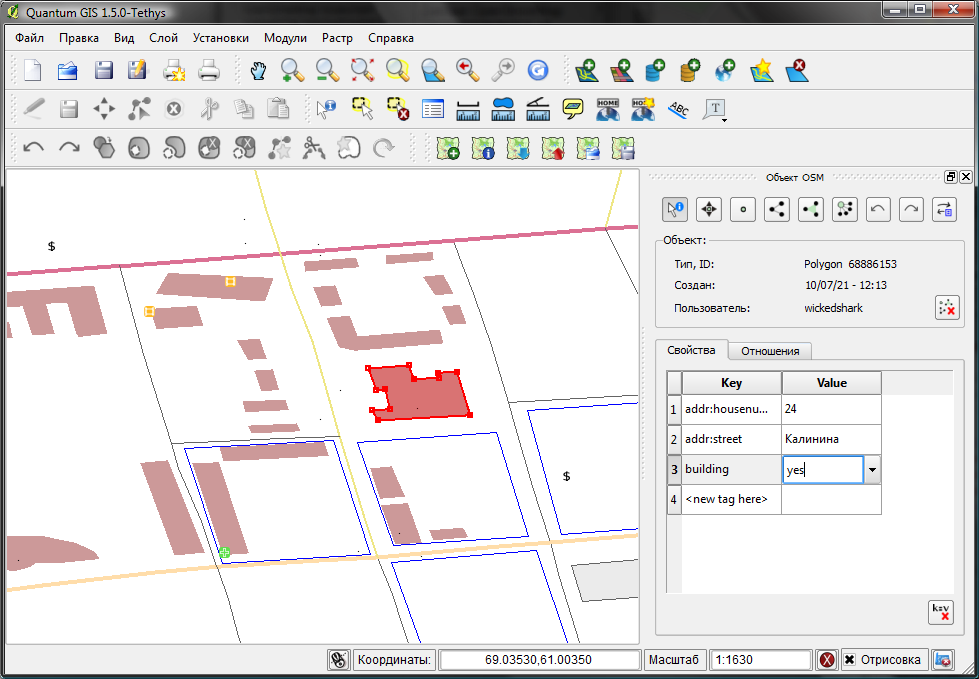
\includegraphics[clip=true, width=12cm]{osm_changefeaturetag}
   \caption{Cambiare l'etichetta di un elemento OSM \wincaption}\label{fig:osmchfeattag}
\end{figure}

Per cambiare il valore di un'etichetta, fare doppio-click in una casella della colonna 'Value' 
ed inserire o selezionare il nuovo valore. Per rimuovere un'etichetta selezionarne la riga 
e cliccare su \button{Remove selected tags} in fondo alla tabella sulla destra.

Per inserire una nuova etichetta, inserire chiave e valore nell'ultima riga della tabella, 
dove appare la scritta '<next tag value>': non è possibile cambiare la chiave di un coppia 
'key/value' esistente. 
Una serie di menu a tendina permettono di selezionare tra i valori tipici di una specifica chiave.

\minisec{Creare punti}

Per creare un nuovo punto, cliccare su \toolbtntwo{osm_createPoint}{Crea punto}, quindi sulla mappa.
Se il cursore del mouse passa sopra qualche elemento della mappa, l'elemento viene evidenziato
e le sue informazioni appaiono nel pannello Elemento OSM; se si clicca sulla mappa quando una linea o 
un poligono sono evidenziati, il nuovo punto viene creato direttamente su questi elementi e 
sarà, quindi, parte di essi (è attiva una funzionalità di snap). 
Non si può creare un punto su un punto esistente: il plugin 
mostrerà il seguente messaggio: 

\begin{figure}[ht]
   \centering
   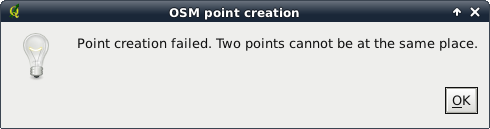
\includegraphics[clip=true, width=8cm]{osm_pointcreation}
   \caption{Messaggio creazione punto OSM \nixcaption}\label{fig:osmpoicreat}
\end{figure}

Se si intende creare un punto molto vicino ad un elemento esistente, ma non su du esso, 
bisogna disabilitare la funzionalità di snap: tenere premuto \keystroke{Ctrl} prima di cliccare sulla 
mappa.

\minisec{Creare linee}

Per creare una nuova linea, cliccare su \toolbtntwo{osm_createLine}{Crea linea}, quindi sulla mappa.
Ogni click con tasto sinistro crea un vertice della nuova linea: per terminare la 
creazione di una linea basta cliccare con il tasto destro.

\textbf{Nota}: Non è possibile creare una linea con meno di due vertici: se si clicca con il tasto 
destro del mouse dopo un solo click con il tasto sinistro, nessuna linea viene creata.

Lo snap è attivo su ogni vertice della mappa - punti del layer di punti e tutte le componenti delle linee 
e dei poligoni. Per disattivare lo snap tenere premuto \keystroke{Ctrl} prima di cliccare sulla 
mappa.

\minisec{Creare poligoni}

Per creare un nuovo poligono, cliccare su \toolbtntwo{osm_createPolygon}{Create polygon}, quindi sulla mappa.
Ogni click con tasto sinistro sarà un vertice del nuovo poligono: per terminare la 
creazione di una linea basta cliccare con il tasto destro.
Non possono essere creati poligoni con meno di tre vertici. 
Lo snap è attivo su ogni vertice della mappa - punti del layer di punti e tutte le componenti delle linee 
e dei poligoni. Per disattivare lo snap tenere premuto \keystroke{Ctrl} prima di cliccare sulla 
mappa. 

\minisec{Spostare un elemento}

Per spostare un elemento cliccare su \toolbtntwo{osm_move}{Muovi elemento}: posizionarsi nella mappa, 
portare il cursore del mouse sull'elemento che si intende spostare, cliccare con il tasto sinistro, 
portare l'elemento nella nuova posizione e cliccare di nuovo con il tasto sinistro. 
Nel caso si fosse selezionato l'elemento sbagliato, non effettuare il secondo click con il tasto sinistro:
cliccando con il tasto destro, l'elemento sarà automaticamente riportato nella sua posizione originale.

Se si sposta una elemento connesso con altri elementi, le loro relazioni non saranno modificate: gli altri 
elementi si autoadatteranno alla nuova posizione dell'elemento cui sono relazionati.

Anche per questa operazione è disponibile la funzionalità di snap:

\begin{itemize}[label=--]
\item quando si muove un punto singolo (cioè che non è parte di una linea/poligono), lo snap è attivo su 
tutti i vertici ed i segmenti in mappa. 
\item quando si muove un punto che è parte di una linea/poligono, lo snap è attivo su 
tutti i vertici ed i segmenti in mappa, tranne i vertici degli elementi di cui il punto fa parte.
\item quando si muove una linea/poligono, lo snap è attivo su tutti i vertici in mappa.
Si noti che il plugin cerca di basare lo snap sui 3 vertici della linea/poligono da spostare più vicini 
al cursore del mouse, altrimenti l'operazione sarebbe estremamente lenta. 
Per disattivare lo snap tenere premuto \keystroke{Ctrl} prima di cliccare sulla 
mappa. 
\end{itemize}

\minisec{Eliminare un elemento}

Per eliminare un elemento selezionarlo con \toolbtntwo{osm_identify}{Informazioni elemento} e cliccare su 
\toolbtntwo{osm_removeFeat}{Rimuovi elemento}. 
Rimuovendo una linea/poligono, vengono rimossi anche 
tutti i punti che ne fanno parte (ma che non fanno parte di altre linee/poligoni).  

Quando si rimuove un punto che fa parte di una linea/poligono, il punto è rimosso e la forma degli 
elementi cui apparteneva si modifica: se il punto da eliminare fa parte di un poligono con soli 
tre vertici, la nuova geometria del poligono avrà due vertici, ma siccome non possono 
esistere poligoni con due vertici, il tipo di elemento viene modificato in linea.
Se il punto faceva parte di una linea, la nuova geometria della linea ha un solo punto e siccome 
non possono esistere linee di un solo punto, il tipo di elemento viene modificato in punto.

\subsection{Modificare le relazioni}\label{editing_osm_relation}

Le relazioni permettono di organizzare più elementi in gruppi ed assegnare loro 
proprietà comuni, in modo da poter modellare qualsiasi oggetto di mappa: es. confini
di una regione come gruppo di 'way' (linee) e 'node' (punti), percorsi di un bus, etc.

Il plugin di QGIS offre un buon supporto alle relazioni OSM.

\minisec{Esaminare una relazione}\label{examrelation}

Per esaminare una relazione, selezionare prima un suo membro, quindi aprire la
scheda \tab{Relazioni} del pannello Elemento OSM, dove saranno elencate tutte 
le relazioni di cui l'elemento è parte. Selezionare una di esse per avere il 
dettaglio delle informazioni. Nella tabella 'Tag relazione' sono visualizzate le 
proprietà della relazione selezionata. Nella tabella 'Membri della relazione'
sono elencati i membri della relazione, cioè tutti gli elementi connessi dalla relazione selezionata.
Cliccando su uno dei membri, lo stesso viene evidenziato in mappa.

\minisec{Creare una relazione}

Per creare una relazione è possibile:

\begin{enumerate}
\item Usare il pulsante \toolbtntwo{osm_createRelation}{Crea relazione} del pannello Elemento OSM.
\item Usare il pulsante \toolbtntwo{osm_addRelation}{Aggiungi relazione} nella scheda \tab{Relazioni} 
del pannello Elemento OSM.
\end{enumerate}

Apparirà la finestra di dialogo \dialog{Crea una relazione OSM}. Nel secondo caso, l'elemento 
selezionato è automaticamente considerato il primo membro della relazione ed il dialogo è precompilato 
in minima parte.
Selezionare un tipo di relazione, tra quelle predefinite e disponibili nel menu a tendina, o crearne 
una nuova, quindi inserire le etichette della relazione e selezionare i suoi membri.

Una volta selezionato un tipo di relazione, cliccare su \toolbtntwo{osm_generateTags}{Genera i tags}: 
nel riquadro 'Proprietà' saranno elencate le etichette tipiche per il tipo di relazione.
Inserire i valori nella colonna 'Value' 

Per inserire i membri della relazione è possibile scrivere direttamente i loro identificatori, tipi e ruoli 
oppure usare il pulsante \toolbtntwo{osm_identify}{Scegli un membro sulla mappa}. 
Cliccare su \button{Crea} per terminare l'operazione.

\minisec{Modificare una relazione}

Per modificare una relazione, selezionarla come visto nella precedente sezione 'Esaminare una relazione', 
quindi cliccare su \toolbtntwo{osm_editRelation}{Modifica relazione}. Nella finestra di dialogo 
\dialog{Edit OSM relation} è possibile modificare le etichette, i membri o il tipo di relazione: 
cliccare su \button{Save} per salvare i cambiamenti.

\subsection{Scaricare dati OSM}

Per scaricare dati dal server di OpenStreetMap cliccare su \toolbtntwo{osm_download}{Download OSM data}. 
Qualora il pulsante non fosse disponibile nell'interfaccia di QGIS, la barra degli strumenti OpenStreetMap 
potrebbe essere disattivata: per attivarla cliccare su \mainmenuopt{Visualizza} \arrow
\mainmenuopt{Barre degli Strumenti} \arrow \dropmenuopt{OpenStreetMap}. La finestra di dialogo 
\dialog{Download dati OSM} fornisce le seguenti funzionalità:

\begin{figure}[ht]
   \centering
   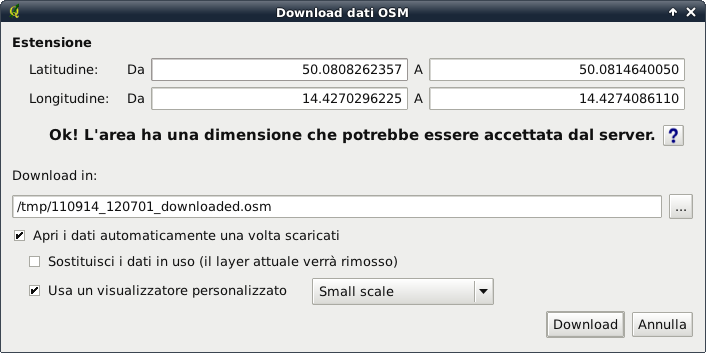
\includegraphics[clip=true, width=8cm]{osm_downloaddialog}
   \caption{Finestra di dialogo Download dati OSM \nixcaption}\label{fig:osmdownload}
\end{figure}

\begin{description}
\item \textbf{Estensione}: permette di impostare l'area da scaricare, indicando le coordinate i gradi di
latitudine e longitudine. Prestare attenzione a non indicare un'area troppo vasta: il server di 
OpenStreetMap ha delle restrizioni sulla quantità di dati scaricabili. Ulteriori informazioni 
sull'estensione dei dati sono disponibili cliccando su \toolbtntwo{osm_questionMark}{?}.
\item \textbf{Download in}: il percorso alla cartella in cui salvare i dati. 
\item \textbf{Apri i dati automaticamente una volta scaricati}: permette di definire se caricare i dati non 
appena scaricati. Se non si desidera caricare subito i dati disattivare l'opzione: i dati potranno 
essere caricati in un secondo momento cliccando su \toolbtntwo{osm_load}{Load OSM from file}.
\item \textbf{Sostituisci i dati in uso}: l'opzione è disponibile solo se lo è anche la precedente. 
Attivando l'opzione, i dati scaricati andranno a sostituire quelli presenti nella vista mappa di QGIS: i 
layer presenti nella vista mappa saranno rimossi. Quando si avvia QGIS e si scaricano dati OSM per la 
prima volta, l'opzione non è attiva, in quanto non c'è nulla da sostituire.
\item \textbf{Usa un visualizzatore personalizzato}: l'opzione è attiva solo se lo è anche 
\radiobuttonon{Apri i dati automaticamente una volta scaricati}. Determinare quanti dettagli della mappa 
visualizzare (scelta tra Small scale, Medium scale, Large scale). Usare \button{Small scale} per 
visualizzare il massimo dei dettagli. QGIS \CURRENT non supporta il cambiamento dinamico del visualizzatore.
\end{description}

Cliccare su \button{Download} per avviare il processo: una finestra di dialogo mostra la percentuale 
di download. Qualora ci fossero errori, un'ulteriore finestra mostra il tipo di errore occorso.
A completamento del download, le varie finestre di chiudono automaticamente.

\subsection{Caricare i dati sul server OSM}

Il caricamento dei dati sul server OSM riguarda i dati visualizzati nella vista mappa di QGIS: prima di caricare 
i dati assicurarsi che nella vista mappa siano visualizzati i dati corretti. 

Per caricare i dati sul server OSM, cliccare su \toolbtntwo{osm_upload}{Upload OSM data}. 
Qualora il pulsante non fosse disponibile nell'interfaccia di QGIS, la barra degli strumenti OpenStreetMap 
potrebbe essere disattivata: per attivarla cliccare su \mainmenuopt{Visualizza} \arrow
\mainmenuopt{Barre degli Strumenti} \arrow \dropmenuopt{OpenStreetMap}. Verrà aperta la finestra di dialogo 
\dialog{Invia dati a OSM}.

\begin{figure}[ht]
   \centering
   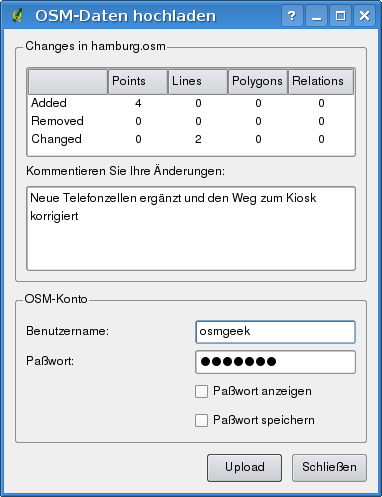
\includegraphics[clip=true, width=8cm]{osm_uploaddialog}
   \caption{Finestra di dialogo Invia dati a OSM \nixcaption}\label{fig:osmupload}
\end{figure}

In alto nella finestra è possibile verificare la correttezza dei dati che si sta caricando. Nella tabella 
vengono elencati i cambiamenti che si stanno apportando, mentre sono riportate separatamente delle 
statistiche per ogni tipo di elemento.

In 'Commenti alle tue modifiche' è possibile inserire delle informazioni aggiuntive: elencare brevemente 
le modifiche apportate.
Compilare i campi 'Account OSM' per l'autenticazione sul server: per creare un account OSM visitare 
la pagina web \url{http://www.openstreetmap.org}. Infine, cliccare \button{Upload} per avviare il processo 
di invio dei dati.

\subsection{Salvare i dati OSM}

Per salvare dati in un file XML, cliccare su \toolbtntwo{osm_save}{Save OSM to file}. 
Qualora il pulsante non fosse disponibile nell'interfaccia di QGIS, la barra degli strumenti OpenStreetMap 
potrebbe essere disattivata: per attivarla cliccare su \mainmenuopt{Visualizza} \arrow
\mainmenuopt{Barre degli Strumenti} \arrow \dropmenuopt{OpenStreetMap}. Verrà aperta la finestra di dialogo 
\dialog{Salva OSM}.

\begin{figure}[ht]
   \centering
   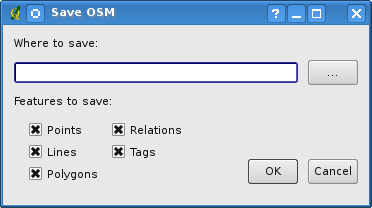
\includegraphics[clip=true, width=8cm]{osm_savedialog}
   \caption{Finestra di dialogo Salva OSM \nixcaption}\label{fig:osmsave}
\end{figure}

Selezionare gli elementi da salvare ed il file i cui salvarli e cliccare su \button{Ok} per avviare il 
processo. La versione OSM del file XML è la 0.6: gli elementi non vengono ordinati. 

Si noti che verranno salvati i soli dati della vista mappa. Linee e poligoni sono salvati interamente, 
anche se sono visualizzati solo in parte: per ogni linea/poligono anche tutti i suoi membri sono salvati.

\subsection{Importare dati in OSM}

Per importare dati in OSM da un layer vettoriale non-OSM seguire le seguenti istruzioni: selezionare 
i dati OSM, cliccando su uno dei layer, e cliccare su \toolbtntwo{osm_import}{Import data from a layer}. 
Qualora il pulsante non fosse disponibile nell'interfaccia di QGIS, la barra degli strumenti OpenStreetMap 
potrebbe essere disattivata: per attivarla cliccare su \mainmenuopt{Visualizza} \arrow
\mainmenuopt{Barre degli Strumenti} \arrow \dropmenuopt{OpenStreetMap}. 
Potrebbe apparire la seguente finestra di dialogo:

\begin{figure}[ht]
   \centering
   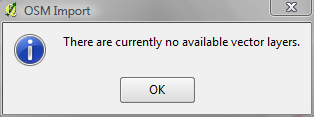
\includegraphics[clip=true, width=8cm]{osm_importdialog}
   \caption{Finestra di errore OSM Import\nixcaption}\label{fig:osmimportmessage}
\end{figure}

La finestra informa che non sono disponibili in QGIS layer vettoriali da cui importare dati. Caricare un layer 
vettoriale e riprovare: ricordarsi di selezionare il layer OSM in legenda:

\begin{figure}[ht]
   \centering
   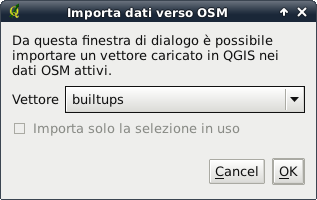
\includegraphics[clip=true, width=5cm]{osm_importtoosmdialog}
   \caption{Finestra di dialogo Importa dati verso OSM \nixcaption}\label{fig:osmimporttoosm}
\end{figure}

Cliccare su \button{OK} per avviare il processo o su \button{Cancel} per annullare.

\FloatBarrier
